\documentclass[12pt%
%,draft%
,xcolor=table
,aspectratio=169%
]{beamer}
%
\usepackage{fontspec}
\defaultfontfeatures{Ligatures=TeX}
%\setsansfont{Liberation Sans}
\usepackage{polyglossia}
\setdefaultlanguage{ngerman}
% Alternative template for talks of the Freie Universität Berlin.
% Created by Leonard R. König, <leonard.koenig@fu-berlin.de> following the
% guidelines on www.fu-berlin.de/cd
%
% (c) Leonard König, CC BY 4.0
%
% This template was written against UTF-8 capable LaTeX engines, specifically
% LuaLaTeX.

% Trying to get rather close to the ppt/odp template:
%  http://www.fu-berlin.de/sites/cd/downloads_container/PowerPoint_Praesentation_Anleitung.pdf

%%% font styles
\setbeamerfont{frametitle}{series=\bfseries}
\setbeamerfont{footline}{series=\bfseries}
\setbeamerfont{headline}{series=\bfseries}
\setbeamerfont{alerted text}{series=\bfseries}
%%%

% colordefs
\definecolor{fu_darkblue}{RGB}{0,51,102}
\definecolor{fu_seablue}{RGB}{0,102,204}
\definecolor{fu_lightblue}{RGB}{204,214,224}
\definecolor{fu_green}{RGB}{153,204,0}
\definecolor{fu_lightgrey}{RGB}{128,128,128}
\definecolor{fu_grey}{RGB}{95,95,95}
%
\definecolor{fu_red}{RGB}{204, 0, 0} % red text (used by \alert)
%%% end colordefs

%%% colors
\setbeamercolor*{title}{fg=fu_darkblue}
\setbeamercolor*{subtitle}{fg=fu_seablue}
\setbeamercolor*{frametitle}{fg=fu_darkblue}
\setbeamercolor*{footline}{fg=fu_grey,bg=fu_lightblue}
\setbeamercolor*{headline}{fg=fu_grey}

\setbeamercolor*{normal text}{fg=black}
\setbeamercolor*{alerted text}{fg=fu_red}
\setbeamercolor*{example text}{fg=fu_green}
\setbeamercolor*{structure}{fg=fu_darkblue}

\setbeamercolor*{block title}{fg=white,bg=black!50}
\setbeamercolor*{block title alerted}{fg=white,bg=black!50}
\setbeamercolor*{block title example}{fg=white,bg=black!50}

\setbeamercolor*{block body}{bg=black!10}
\setbeamercolor*{block body alerted}{bg=black!10}
\setbeamercolor*{block body example}{bg=black!10}

\setbeamercolor{bibliography entry author}{fg=fu_darkblue}

\setbeamercolor{item}{fg=fu_darkblue}
\setbeamercolor{navigation symbols}{fg=fu_lightgrey,bg=fu_grey}
%%% end colors

%%% title page
% Display logo (if exists) and right next to it, put our title + subtitle
\defbeamertemplate*{title page}{fu_titlepage}
{%
	\hskip .3\textheight
	\begin{minipage}[.4\textheight]{\textwidth}
		\begin{minipage}[.4\textheight]{0.25\textwidth}
			\inserttitlegraphic
		\end{minipage}%
		\begin{minipage}[.4\textheight]{0.75\textwidth}
			\begin{beamercolorbox}{title}
				\usebeamerfont{title}\inserttitle\par%
			\end{beamercolorbox}
			\vfill
			\ifx\insertsubtitle
				\@empty%
			\else
				\begin{beamercolorbox}{subtitle}
					\usebeamerfont{subtitle}\insertsubtitle\par
				\end{beamercolorbox}
			\fi
		\end{minipage}
	\end{minipage}%
	\hskip .3\textheight
}
%%% end title page

%%% headline
% display title, author and institute on the left;
% logo on the right.
\newcommand{\headlinetext}
{%
	\inserttitle\\[0.3em]%
	\insertauthor, %
	\insertshortinstitute
}
\newlength{\headlinewidth}
\setlength{\headlinewidth}{\paperwidth}
\addtolength{\headlinewidth}{-2\marginparsep}
\setbeamertemplate{headline}
{%
	\begin{beamercolorbox}[wd=\paperwidth]{headline}%
		\vskip5pt
		{\hspace*{\marginparsep}}%
		\parbox{.5\headlinewidth}
		{%
			\usebeamertemplate{title in head/foot}%
			\headlinetext%
		}%
		\begin{minipage}{.5\headlinewidth}%
			\hfill\usebeamertemplate*{logo}
		\end{minipage}%
		{\hspace*{\marginparsep}}%
	\end{beamercolorbox}%
}
%%% end headline

%%% footline
% title + date on the left, frame number on the right
\newcommand{\footlinetext}
{%
	\usebeamerfont{shorttitle}\insertshorttitle, %
	\usebeamerfont{shortdate}\insertshortdate
}
\setbeamertemplate{footline}
{%
	\begin{beamercolorbox}{footline}
		\vskip2pt
		\hspace{\marginparsep}%
		\footlinetext\hfill%
		\insertframenumber%
		\hspace{\marginparsep}
		\vskip2pt
	\end{beamercolorbox}%
}
%%% end footline

% don't use default templates for sidebars
\setbeamertemplate{sidebar right}{}
\setbeamertemplate{sidebar left}{}
\setbeamertemplate{title page}[fu_titlepage]
\usepackage{amsmath}
\usepackage{amsfonts}
\usepackage{amssymb}
\usepackage{graphicx}
\usepackage{algorithm}
\usepackage[noend]{algpseudocode}
%\usepackage{algorithmic}
\usepackage{tikz}
\usetikzlibrary{arrows,shapes,automata,petri,positioning,calc}
\usepackage{graphicx}
\usepackage{subfig}
\usepackage{pgfplots}
\usepackage{ stmaryrd }
\usepackage[normalem]{ulem}
\usepackage{circuitikz}
\usepackage{bohr}
\usepackage{csquotes}


\setbeamercolor{block title}{use=structure,fg=white,bg=structure.fg!75!black}
\setbeamercolor{block body}{parent=normal text,use=block title,bg=block title.bg!10!bg}


\usepackage{expl3}

\ExplSyntaxOn
\cs_new:Npn \displayasdecimal#1 {(#1) \sb {10}}
\cs_new:Npn \displayasoctal #1 {(\int_to_oct:n{#1}) \sb 8}
\cs_new:Npn \displayasbinary #1 {(\int_to_bin:n{#1}) \sb 2}
\ExplSyntaxOff

\newcounter{divline}
\def\rlwd{.5pt} \def\rlht{\dimexpr\dp\strutbox+\ht\strutbox} \def\rldp{.75ex}
\newcommand\mydiv[3][\relax]{%
  \ifx\relax#1\stepcounter{divline}\else\setcounter{divline}{#1}\fi%
  \mbox{}\hspace{\thedivline\dimexpr1ex}#2~\setbox0=\hbox{~$#3$}%
  \dumbstackengine{-\rlwd}{\rule[-\rldp]{\rlwd}{\rlht}~#3}{\rule{\dimexpr4pt+\wd0}{\rlwd}}%
}
\def\remainder#1{\stepcounter{divline}%
  \mbox{}\hspace{\dimexpr1ex+\thedivline\dimexpr1ex}~#1\setcounter{divline}{0}}
\makeatletter
\global\newlength\@stackedboxwidth
\newlength\@boxshift
\newsavebox\@addedbox
\newsavebox\@anchorbox
\newcommand*\dumbstackengine[3]{%
    \sbox{\@anchorbox}{$#2$}%
    \sbox{\@addedbox}{$#3$}%
    \setlength{\@stackedboxwidth}{\wd\@anchorbox}%
      \ifdim\wd\@addedbox>\@stackedboxwidth%
        \setlength{\@stackedboxwidth}{\wd\@addedbox}%
      \fi%
        \setlength{\@boxshift}{\dimexpr-\dp\@anchorbox -\ht\@addedbox -#1}%
        \usebox{\@anchorbox}%
        \hspace{-\wd\@anchorbox}%
        \raisebox{\@boxshift}{\usebox{\@addedbox}}%
        \hspace{-\wd\@addedbox}%
        \hspace{\@stackedboxwidth}%
}

\newcommand\decbin[9]{%
\par\smallskip
\makebox[3cm][r]{$#1$\ }\fbox{#2}\,\fbox{#3}\,\fbox{#4}\,\fbox{#5}\,\fbox{#6}\,\fbox{#7}\,\fbox{#8}\,\fbox{#9}\par}


\def\unsignedbytecalc#1{%
\par\smallskip
\noindent$#1_{10}$\par
\smallskip
\gdef\result{}%
$\left.\begin{array}{r@{\quad}|c}\udbc{#1}\end{array}\right\}\result$\par}

\def\udbc#1{%
\ifnum#1=\z@
\expandafter\@gobble
\else
\expandafter\@firstofone
\fi
{2)\!\underline{\,#1}&\edef\r{\ifodd#1 1\else 0\fi}\r\xdef\result{\r\result}\\
\expandafter\udbc\expandafter{\the\numexpr(\ifodd#1 #1-1\else#1\fi)/2\relax}%
}}


\author{Benjamin Tröster}
\title[Zeichenkodierung]{Zeichenkodierung}
%\subtitle[Addition \& Subtraktion]{Addition \& Subtraktion}
%\pgfdeclareimage{titlegraphic}{../res/dwarf_logo2.png}
%\titlegraphic{\pgfuseimage{titlegraphic}}
%\date{}
%\subject{}
%
% FU settings
\institute[HTW Berlin]{Hochschule für Technik und Wirtschaft Berlin}
%\pgfdeclareimage[height=0.9cm]{logo}{../res/dwarf_logo}
%\logo{\pgfuseimage{logo}}
%
\usepackage[
backend=biber,
citestyle=alphabetic,bibstyle=authoryear
]{biblatex}
\addbibresource{sources.bib}


\begin{document}

\begin{frame}
\titlepage
\end{frame}

\begin{frame}{Fahrplan}
\tableofcontents[hideothersubsections]
\end{frame}

\section{Zeichenkodierung}

\begin{frame}{Zeichenkodierung}
\begin{itemize}
	\item Um Text auf einem Computer darzustellen, muss jeder Buchstabe binär kodiert werden
	\item Je nachdem wie viele Bits pro Zeichen verwendet werden, können unterschiedlich viele verschiedene Zeichen abgelegt werden
	\item Beispiel:
	\begin{itemize}
		\item 7 Bits: $2^7 = 128$ verschiedene Zeichen
		\item 8 Bits: $2^8 = 256$ verschiedene Zeichen
		\item 16 Bits: $2^{16} = 65536$ verschiedene Zeichen
	\end{itemize}
 \end{itemize}
\end{frame}

\subsection{ASCII-Code}
\begin{frame}{ASCII-Code}
\begin{itemize}
	\item Der ASCII-Code (American Standard Code for Information Interchange) ist eine 7-Bit-Zeichenkodierung, die 1963 von der American Standards Association (ASA) beschlossen wurde
	\item Ein Zeichen wird jedoch immer als 1 Byte (=8 Bits) abgelegt, d.h. das höchstwertige (8.) Bit ist immer Null
	\item Insgesamt gibt es 128 Zeichen, davon 95 druckbare und 33 Steuerzeichen
\end{itemize}
\end{frame}

\begin{frame}{ASCII-Code}
\begin{itemize}
	\item In folgender Tabelle sind alle 128 ASCII-Zeichen angegeben
	\begin{figure}
	\center
	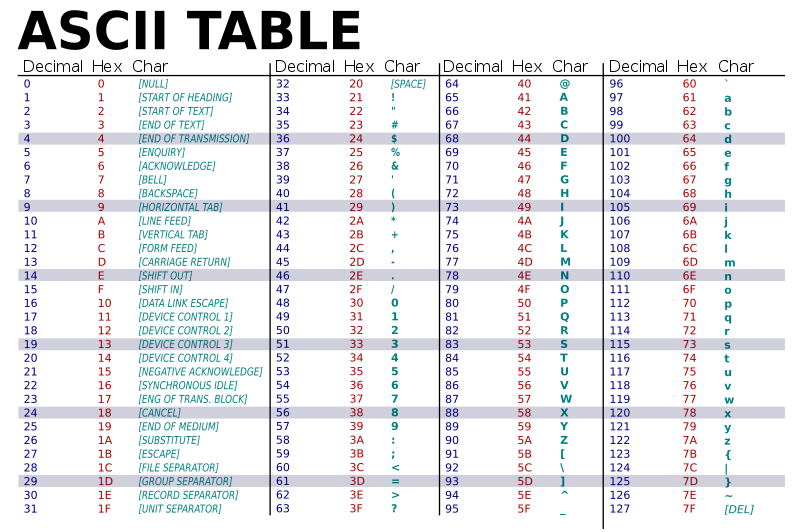
\includegraphics[scale=0.3]{pictures/ascii}
	\end{figure}
	\item Beispiel: Das Zeichen \enquote{A} hat den Hexadezimalwert $41_{16}$ $41_{16} = 01000001_2 = 65_{10}$
\end{itemize}
\end{frame}

\begin{frame}{ASCII-Code}
\begin{itemize}
	\item Die Steuerzeichen stammen aus einer Zeit, in der der ASCII-Code zur Steuerung von Fernschreibern (elektrisch angesteuerte Schreibmaschinen) verwendet wurde
	\item Heutzutage habe viele dieser Steuerzeichen ihre Bedeutung verloren
	\item Wichtig ist eigentlich nur noch das Steuerzeichen für eine neue Zeile: \enquote{LF} (Line Feed, ASCII $0A_{16}$
	\item Beim Betriebssystem Windows muss dem \enquote{Line Feed} Zeichen allerdings noch ein \enquote{Carriage Return} vorangestellt werden: \enquote{CR LF} (=ASCII $0D_{16} 0A_{16}$)
\end{itemize}
\end{frame}

\subsection{ISO 8859}
\begin{frame}{ISO 8859}
\minipage{0.45\textwidth}
\begin{itemize}
	\item Bei der ASCII-Codierung werden nur 7 der 8 Bits eines Bytes genutzt
	\item Der restliche Zahlenbereich (128 bis 255) kann also für weitere Zeichen verwendet werden
	\item Die International Organization for Standardization definiert in ISO 8859 insgesamt 15 ASCII-Erweiterungen
	\item ISO 8859-1 enthält z.B. die für uns in Deutschland wichtigen Buchstaben: ä, ü, ö, ß
\end{itemize}
\endminipage \hfill
\minipage{0.45\textwidth}%

\begin{table}[]
\resizebox{\columnwidth}{!}{%
\begin{tabular}{|l|l|}
\hline
ISO 8859-1 	& Westeuropäisch (Latin-1) \\ \hline
ISO 8859-2 & Mitteleuropäisch (Latin-2) \\ \hline
ISO 8859-3 &	Südeuropäisch (Latin-3) \\ \hline
ISO 8859-4 &	Nordeuropäisch (Latin-4) \\ \hline
ISO 8859-5 &	Kyrillisch \\ \hline
ISO 8859-6 &	Arabisch\\ \hline
ISO 8859-7 &	Griechisch\\ \hline
ISO 8859-8 &	Hebräisch\\ \hline
ISO 8859-9 &	Türkisch (Latin-5)\\ \hline
ISO 8859-10& 	Nordisch (Latin-6)\\ \hline
ISO 8859-11& 	Thai\\ \hline
ISO 8859-12& 	verworfen\\ \hline
ISO 8859-13& 	Baltisch (Latin-7)\\ \hline
ISO 8859-14& 	Keltisch (Latin-8)\\ \hline
ISO 8859-15& 	Westeuropäisch (Latin-9)\\ \hline
ISO 8859-16& 	Südosteuropäisch (Latin-10)\\ \hline
\end{tabular}
}
\end{table}
\endminipage
\end{frame}

\subsection{Unicode}

\begin{frame}{Unicode}
\begin{itemize}
	\item Bei der Verwendung von ISO 8859 zum Austausch von Texten kommt es immer wieder zu fehlerhaften Darstellungen von Zeichen. Dies passiert leicht, wenn Sender und Empfänger nicht die gleiche ISO 8859-x Norm zur Dekodierung verwenden
	\item Außerdem sind in ISO 8859 längst nicht alle Schriftzeichen aus den unterschiedlichsten Kulturkreisen erfasst
	\item Die Bestrebung des Unicode ist es, eine einzige universelle Kodierung zu definieren, die alle relevanten Zeichen enthält
	\item Der Unicode wurde von der ISO als ISO-10646 standardisiert
\end{itemize}

\end{frame}

\begin{frame}{Unicode}
\begin{itemize}
	\item Der Unicode besteht aus 17 Ebenen (darstellbar mit 5 Bits)
	\item Jede Ebene hat 16 Bits und kann damit theoretisch $2^{16}=65536$ Zeichen kodieren
	\item Insgesamt kann ein Unicode also 5+16=21 Bits benötigen
	\item Die meisten aktuell verwendeten Zeichen sind in Ebene $0$, der Basic Multilingual Plane (BMP), zu finden
	\item Ein Unicode Zeichen wird üblicherweise als ein \enquote{U+} und einer Hexadezimalzahl mit mindestens 4 Stellen angegeben
	\item Beispiele:
	\begin{itemize}
		\item $U+00E4$ für das ä
		\item $U+00A9$ für die Copyright Symbol \symbol{"00A9} 
	\end{itemize}
\end{itemize}

\end{frame}

\begin{frame}{Unicode Aufbau}
\begin{itemize}
	\item Die Kodierung aller möglichen Schriftzeichen ist ein andauernder Prozess, d.h. die Anzahl der Zeichen wächst ständig
	\item Ein Problem bei der Darstellung ist, dass die meisten Schriftarten nur eine kleine Untermenge der im Unicode definierten Zeichen bereit halten
    \item Ist ein Zeichen in einer Schrift nicht vorhanden, wird oftmals einfach ein Zeichen aus einer anderen Schriftart eingefügt
    \item Die Webseite \url{http://www.decodeunicode.org/} hat es sich zur Aufgabe gemacht, alle aktuell im Unicode kodierten Zeichen darzustellen
\end{itemize}

\end{frame}

\begin{frame}{Unicode}
\begin{itemize}
	\item Beim Entwurf des Unicode wurde auf Kontinuität wert gelegt
	\item Aus den 21 Bits des Unicodes entsprechen die ersten 7 Bits dem ASCII-Code und die ersten 8 Bits der ASCII-Erweiterungen ISO 8859-1 (Latin 1)
	\begin{figure}
	\center
	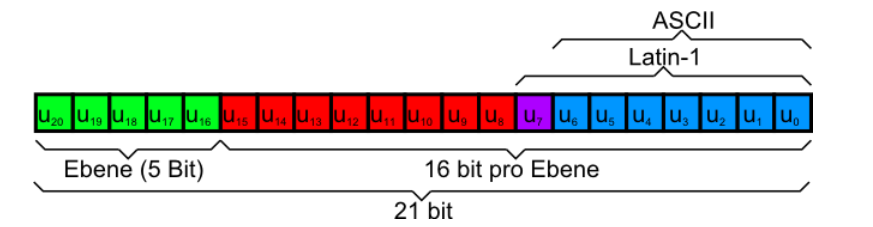
\includegraphics[scale=0.4]{pictures/unicode1}
	\end{figure}
\end{itemize}

\end{frame}

\subsection{UTF}

\begin{frame}{UTF}
\begin{figure}
\center
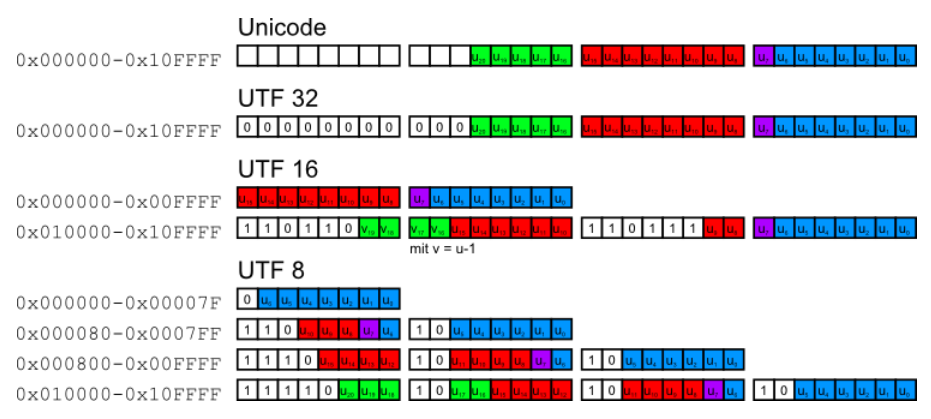
\includegraphics[scale=0.3]{pictures/utf}
\end{figure}
\begin{itemize}
	\item Zur Kodierung von Unicode-Zeichen wird meistens das UTF \enquote{Universal Transformation Format} verwendet
	\item UTF-32 kodiert jedes Unicode-Zeichen mit 32 Bits, indem es die 21 Unicode Bits mit Nullen auffüllt
	\item UTF-16 kodiert alle Bits der Basic Multilingual Plane (BMP) mit 16 Bits, nur für die anderen Ebenen werden 32 Bits benötigt
\end{itemize}
\end{frame}

\begin{frame}{UTF-8}
\begin{figure}
\center
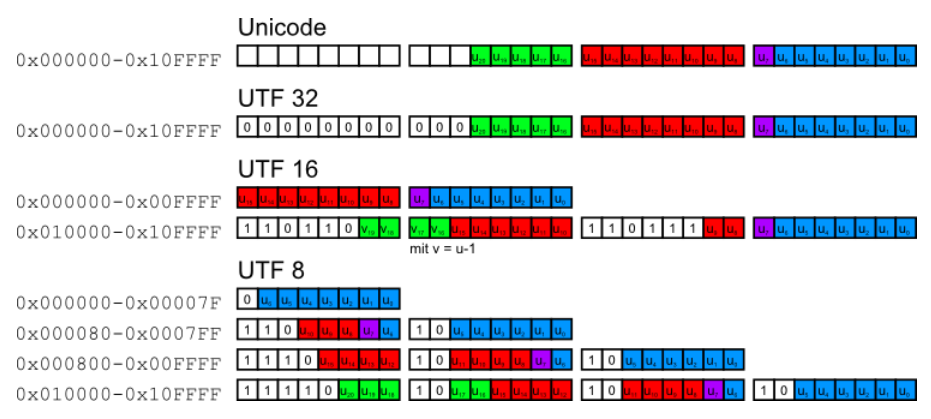
\includegraphics[scale=0.3]{pictures/utf}
\end{figure}
\begin{itemize}
	\item UTF-8 kodiert die ersten 7 Unicode Bits (entspricht ASCII) mit 8 Bits, die ersten 11 Unicode Bits mit 16 Bits, usw.
	\item Ein UTF-8 kodierter Text, der nur ASCII Zeichen enthält, ist demnach vollständig mit ASCII kompatibel
    \item UTF-8 ist heutzutage (besonders im Internet) weit verbreitet (Quasi-Standard der Zeichenkodierung)

\end{itemize}
\end{frame}



\section*{Quellen}
\appendix
\begin{frame}[allowframebreaks]
  \frametitle<presentation>{Quellen}
\printbibliography
\end{frame}
\end{document}